\chapter{Graphs of Quadratic Expressions}

Identify the vertex and axis of symmetry for each.

\begin{multicols}{3}
\begin{enumerate}   
    \item $y = 5x^2 - 15x + 7$
    \item $y = x^2 + 8x - 1$
    \item $y = \frac{1}{4}\left(x+3\right)^2 + 1$
\end{enumerate} \setcounter{Review}{\value{enumi}}
\end{multicols}

Write each of the following in general, $y = ax^2 + bx + c$, form.

\begin{multicols}{3}
\begin{enumerate}   \setcounter{enumi}{\value{Review}}
    \item $y = (x-7)^2 + 4$
	\item $y = -3(x+2)^2-5$
	\item $y = \frac{1}{4}(x-7)^2+1$
\end{enumerate} \setcounter{Review}{\value{enumi}}
\end{multicols}

Write each of the following in $y = a(x-h)^2 + k$ and $y = ax^2 + bx + c$ form.

\begin{multicols}{2}
\begin{enumerate}   \setcounter{enumi}{\value{Review}}
    \item \mbox{} \newline\\
	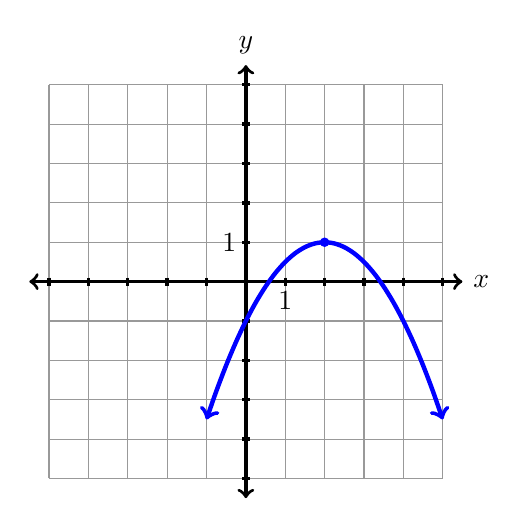
\begin{tikzpicture}[scale=0.5]
	\draw [gray!80] (-5,-5) grid (5,5);
	\draw[<->, very thick] (-5.5,0) -- (5.5,0) node [right] {$x$};
	\draw[<->, very thick] (0,-5.5) -- (0,5.5) node [above] {$y$};
	\foreach \x in {-5,-4,...,5}
	\draw[very thick] (\x, 0.1) -- (\x, -0.1);
	\foreach \y in {-5,-4,...,5}
	\draw[very thick] (0.1,\y) -- (-0.1,\y);
	\node at (1,0) [below] {$1$};
	\node at (0,1) [left] {$1$};
	\draw[<->,ultra thick, color=blue, smooth, domain=-1:5] plot (\x, {-0.5*(\x-2)*(\x-2)+1});
	\draw[color=blue,fill=blue] (2,1) circle [radius=3pt];
	\end{tikzpicture}
	
	\item \mbox{} \newline\\
	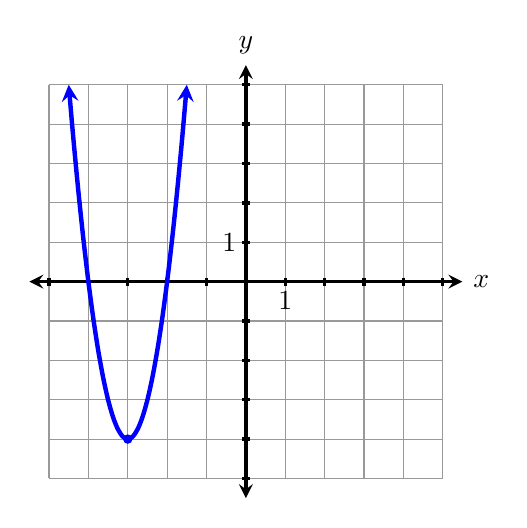
\begin{tikzpicture}[>=stealth, scale=0.5]
	\draw [gray!80] (-5,-5) grid (5,5);
	\draw[<->, very thick] (-5.5,0) -- (5.5,0) node [right] {$x$};
	\draw[<->, very thick] (0,-5.5) -- (0,5.5) node [above] {$y$};
	\foreach \x in {-5,-4,...,5}
	\draw[very thick] (\x, 0.1) -- (\x, -0.1);
	\foreach \y in {-5,-4,...,5}
	\draw[very thick] (0.1,\y) -- (-0.1,\y);
	\node at (1,0) [below] {$1$};
	\node at (0,1) [left] {$1$};
	\draw[<->,ultra thick, color=blue, smooth, domain=-4.5:-1.5] plot (\x, {4*(\x+3)*(\x+3)-4});
	\draw[color=blue,fill=blue] (-3,-4) circle [radius=3pt];
\end{tikzpicture}
\end{enumerate} \setcounter{Review}{\value{enumi}}
\end{multicols}

\newpage


\section{Answer Key}

\begin{enumerate}
	\item Vertex: $\left(\frac{3}{2}, -\frac{17}{4}\right)$; \quad Axis of Symmetry: $x = \frac{3}{2}$
    \item Vertex: $(-4,-17)$; \quad Axis of Symmetry: $x = -4$
    \item Vertex: $(-3,1)$; \quad Axis of Symmetry: $x = -3$
    
    \item $y = x^2 - 14x + 53$
    \item $y = -3x^2-12x-17$
    \item $y = \frac{1}{4}x^2-\frac{7}{2}x+\frac{53}{4}$
    
    \item $y = -\frac{1}{2}(x-2)^2+1 = -\frac{1}{2}x^2+2x-1$
    \item $y = 4(x+3)^2-4 = 4x^2+24x+32$
\end{enumerate}